\chapter{Literature Review} \label{ch2:Literature}

\section{Introduction}

This chapter presents the literature review about soft robotic applications implemented in human assistance in the following order. Firstly, the field of Soft Robotics is introduced. Secondly, an overview of many soft robotic applications for human assistance is provided. Thirdly, the terminology around the biomechanics of the human lower limb is introduced. Fourthly, the mechanical properties of the human muscle-tendon component are described. Fifthly, the modelling tools currently being implemented for the prediction of the mechanical properties of soft materials is investigated. Lastly, resulting from the extensive literature review, the gaps on the body of knowledge are identified and described in the summary section of this chapter.

\section{The Field of Soft Robotics}

The field of Soft Robotics deals with the implementation of soft and deformable materials in traditional robotic applications. The interest in this field has increased in the past decade. The latter is due to the outstanding progress in manufacturing of soft and smart materials which can be actuated by heat, light, and magnetism. 

The coordination action called RoboSoft, supported by the IEEE Robotics and Automation Society (RAS) and the European Commission, has played a very important role in spreading the awareness of the wide number of soft robotic applications. The RoboSoft committee formally defines the field of Soft Robotics as ``Soft robot/devices that can actively interact with the environment and can undergo `large' deformations relying on inherent or structural compliance'' \cite{laschi2016soft}. The categorization of when a robotic application fall into the field of Soft Robotics depends on the material's Young Modulus, a mechanical property which relates the material's deformation with the amount of stress applied to it; which must be between the range of 10$^{2} - $10$^{6}$ Pascals (Pa). The Young's modulus is usually a measure of a solid material stiffness; a high value refers to a stiff material in the same way as a low value refers to an elastic or soft material. In the context of Soft Robotics, the term compliance is commonly used instead of stiffness since it refers to the adaptability of the material under certain circumstances.

Early applications in Soft Robotics were inspired in nature, by observing that most biological organisms are not rigid, e.g. the human skeleton only contributes with 11\% of an adult's weight, on contrast, the skeletal muscle in our body only contributes with 42\% of the weight \cite{kim2013soft}. This inspiration gave birth to several soft bio-inspired robots, as well as the interest in studying the embodied intelligence of biological organisms. The latter refers to the ability of biological organisms to adapt to different situations by exploding their body morphology and properties. This is one of the main differences between soft and rigid robots. The embodied intelligence of soft robots releases the controller from the task of accurately controlling the position of the robot and of constantly monitoring the working environment; allowing the controller to focus on the execution of commands. This is only possible with the implementation of soft and deformable materials able to automatically adapt to perturbations from the environment, such as uneven terrains and obstacles. Bio-inspired soft robots are now being developed for a broad range of applications, such as locomotion, manipulation, and even replicating biological processes such as digestion. The research done in the field of Soft Robotics has an interesting multidisciplinary potential. For example, the locomotion of caterpillars and snake could be study by building a soft robot which replicates this motion. The knowledge extracted from this could be useful for the development of actuated bendable soft cylinders which ultimately could replace the current rigid tools being used in laparoscopic surgery \cite{rus2015design}.

The mechanical behaviour of soft materials is very difficult to model using traditional mathematical models due to their non-linear, time-dependent and strain-rate-dependent stress response. This great challenge motivated the research in Soft Robotics to develop bio-inspired soft bodies, arms and legs able to perform the task at hand using minimal control. This caused a shift in the traditional design approach for rigid robots from ``rigidity by design, safety by sensors and control'' to the design approach used in soft robots, ``safety by design, performance by control''. The added feature of safety, inherent in most soft robots, allowed the development of physical human-robot interaction (PHRI) applications \cite{filippini2008toward}. Many other challenges faced by this emerging field are: actuation of soft materials, development and implementation of soft sensors into soft robots, control systems capable to deal with the nonlinear behaviour of soft materials, and modelling tools capable to accurately predict the mechanical behaviour of soft materials in real-time \cite{laschi2016soft,trivedi2008soft}. Most of these limitations come from the simple fact that soft robots cannot be considered as a chain of rigid links able to rotate or slide as common robots are, but soft robots are deformable and continuous which means that all the foundation in which Robotics is based on, is not easily transferable to the Soft Robotics field. 

The design and development of soft robots is very challenging, but the potential benefits are many such as: soft robots have the potential of being very dexterous due to the ability of modifying their shape depending on the environment; soft robots can manipulate objects of different shapes, sizes; and most importantly soft robots are safe to interact with humans in the event of an unplanned collision \cite{iida2011soft}. These benefits highlight the potential of soft robotic applications for PHRI such as, orthoses, surgical tools, and wearable devices. This research aims to contribute to the technological advance of Soft Robotics for human assistance applications.

For a long time, humans have pursued the idea of increasing their strength, stamina and speed through different means. Nowadays, this is a reality due to the technological advances on wearable robotic devices, commonly known as robotic exoskeletons. This wearable device was motivated by military applications where a soldier is required to carry a heavy load in its back for a long period of time, ultimately causing him injuries or early fatigue. The robotic exoskeleton is capable to carry a payload and transmit the payload weight to the ground, ideally relieving the wearer from feeling the payload, which allows the wearer to walk greater distances without premature fatigue. The rigid nature of these devices and the big actuators implemented to achieve forces able to enhance humans, impose many limitations, such as, restriction of body movements, interference on subject natural biomechanics and high inertia which impedes the device to follow the subject intentions smoothly, creating a drag feeling \cite{asbeck2014stronger}.

In the field of Soft Robotics, research is being done to develop a soft version of a robotic exoskeleton, formally called soft exosuit, in an attempt to solve the previously mentioned limitations. Soft exosuits are wearable robotic systems meant to be worn in the same way as clothes, by attaching both the actuation and perception systems into a wearable structure, made of textiles, strapped to the human body which will ultimately assist the wearer's motions. Despite the many benefits of this technology, in comparison to the robotic exoskeleton, current developments of soft exosuits are not capable to deliver enough mechanical power to be called an enhancement device. Currently, soft exosuits are categorized as assistive devices. This limitation is inherent from the idea of having a soft wearable device. The accurate delivery of assistive forces generated by the actuators attached to a wearable textile, or directly to the user's body, is very challenging. In a rigid exoskeleton the reaction forces produced by the actuators are sustained by the exoskeleton mechanical frame, but this is not the case in soft exosuits, where the reaction forces must be dissipated through the worn textile attached to the human body, which generates uncomfortable frictions between the user skin and the textile. Nevertheless, the human body naturally possesses regions capable of sustaining high amounts of forces. These regions are used in soft exosuit designs to prevent discomfort, skin injury, and to increase the efficiency of transmitted forces. The latter principle is implemented in \cite{wehner2013lightweight} where a lower limb soft exosuit using pneumatic muscles is developed. The other, most common approach is to fix a wearable soft material to the skin, as in \cite{park2014design,park2011bio} where pneumatic artificial muscles (PAM) were attached to a soft cloth and disposed in such a way that they can mimic the biological musculoskeletal behaviour of a human foot. Among the available soft exosuit developments, few of them implements a closed loop control system, due to the high complexity of dealing with the non-linearity of soft materials. These technologies are described in detail in the following section.

\section{Human Assistance Applications}


The adoption of soft robotics in human assistance applications started with the replacement of rigid and bulky actuators, commonly used in traditional robotic exoskeletons, with soft and flexible actuators such as Pneumatic Artificial Muscles (PAMs) and cable-driven actuators. The latter gave birth to hybrid systems as found in \cite{Noda2014}, where a combination of both the previously mentioned technologies were implemented to overcome the limitation of having high inertia in robotic exoskeletons. The latter work also describes the first attempt of imitating the functionality of the human musculoskeletal system by using cable-driven actuators to transmit the forces created by the PAMs. The latter resembles the functionality of human muscle-tendon component.

During the following years of this adoption process, many rigid devices were implementing soft actuators motivated by the same principle as mentioned earlier. However, in the early stages of soft robotics there was a lack of available soft materials to be implemented as actuators which encouraged researchers to focus mainly on pneumatic actuators \cite{Belforte2014}. As soft robotics gained popularity, researchers in the field of material sciences started to develop new soft materials capable of functioning as actuators. Nonetheless, more research is required to make these new materials safe to be used in soft robotic applications for human assistance. Due to this, current developments in soft exosuits and soft orthoses are built around two well established technologies: pneumatic artificial muscles (PAMs) and cable-driven actuators, commonly based on electric motors, using Bowden cables as the pulling element. In a lesser quantity, technologies such as shape memory alloys (SMAs) and shape memory polymers (SMPs) have been implemented in soft orthoses with unsuccessful results mainly due to their large recovery time which make them unsuitable for human assistance applications. The extent of how these technologies have been implemented in soft robotic applications is presented in the next subsection.

\subsection{Soft Actuation Technologies} \label{sec:SoftActuation}

\subsubsection{Pneumatic Artificial Muscles} \label{sec:PMAs}

The usage of compressed air or gases into engineering applications is called Pneumatics, if an incompressible fluid is used, it is called Hydraulics. In Soft Robotics, the latter principles are translated to expand or contract a soft material to generate forces. Nonetheless, this can also be used to produce different types of locomotion in particular soft robots. As previously mentioned, soft pneumatic actuators were extensively researched in different applications for Soft Robotics. In fact, the usage of soft polymers, such as silicone and elastomers, in combination with PAMs enabled different applications such as legged locomotion \cite{Florez2014}, pneumatic fingers for grasping objects with sensing capabilities \cite{Morrow2015}, soft skin with embedded sensors \cite{Sonar2016,Suh2014} and even implantable cardiac stimulators \cite{Roche2014}. In the field of human assistance, soft pneumatic actuators can be categorized in four main groups: textile muscles, braided fluid muscles (McKibben type), large deformation actuators (LDA) bellows and LDA worms. Only the former three are suitable for some kind of human assistance. However, according to Belforte et al. \cite{Belforte2014}, the most suitable for a biomedical application in rehabilitation are the McKibben muscles due to the advantages described in \Cref{tbl:PMAs_feats}.

\begin{table}[ht!]
  \caption[Main features of pneumatic artificial muscles.]{Main features of pneumatic artificial muscles. Modified from \cite{Belforte2014}.}
  \label{tbl:PMAs_feats}
  \centering
  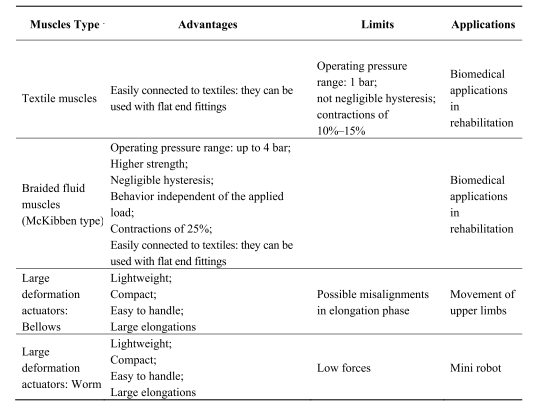
\includegraphics[width=1\textwidth]{Table_PAM_Features.png}
\end{table}

Early works on the assistance of the human lower limbs include the development of a soft orthosis for the foot to treat gait pathologies such as drop-foot \cite{park2011bio,Hamedi2015}. One important aspect of this device is its design, inspired in the musculoskeletal human system. The actuation system was designed to mimic the natural functionality of the muscle-tendon-ligament (\Cref{fig:bio_ankle}). The soft orthosis is powered by Mckibben-type pneumatic actuators. They are attached to a soft support structure consisting of an adapted neoprene knee sleeve and a five toed leather shoe. A total of three off-the-shelf pneumatic muscles assisted the dorsiflexion, eversion and inversion movements of the ankle joint by generating and transmitting tension forces through artificial tendons made of a flexible but non-extensible metal cables (\Cref{fig:bio_ankle_parts}(a)). The tendons were located inside a low-friction material tube to minimize losses during transmission; two of these tendons were anchored to a single point in the foot brace while the other one was anchored in four different points in order to distribute the pulling force, again, mimicking the human body behaviour. The artificial ligaments delivered the same functionality as the biological ones, which is to restrict the movement of the tendons in all the directions other than the one of actuation (\Cref{fig:bio_ankle_parts}(b)). The pneumatic actuators were strategically anchored in two points, at the bottom of the knee sleeve providing nonrestrictive motion of the knee, and at the foot brace.
\begin{figure}[hbt!]
    \centering
    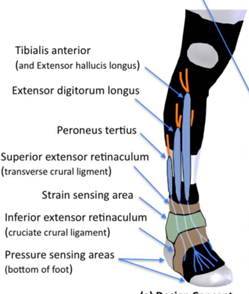
\includegraphics[width=0.4\textwidth]{BioinspiredAnkle.png}
    \caption[Bio-inspired active soft orthosis concept for the treatment of ankle-foot pathologies. From top to bottom: artificial muscles attached to the soft wearable garment, a strain sensor for ankle angle measurements, the tendon-ligament system and pressure sensor for gait cycle detection.]{Bio-inspired active soft orthosis concept for the treatment of ankle-foot pathologies. From top to bottom: artificial muscles attached to the soft wearable garment, a strain sensor for ankle angle measurements, the tendon-ligament system and pressure sensor for gait cycle detection \cite{park2011bio}. }
    \label{fig:bio_ankle}
\end{figure}
\begin{figure}[hbt!]
    \centering
    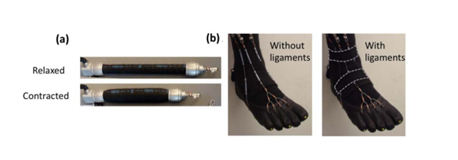
\includegraphics[width=0.8\textwidth]{BioinspiredAnkleParts.png}
    \caption[Soft orthosis components, (a) pneumatic artificial muscle in its relaxed and contracted state, (b) complete tendon-ligament system without ligaments and with ligaments.]{Soft orthosis components, (a) pneumatic artificial muscle in its relaxed and contracted state, (b) complete tendon-ligament system without ligaments and with ligaments \cite{park2011bio}. }
    \label{fig:bio_ankle_parts}
\end{figure}

Another soft orthosis using pneumatic actuation is presented in \cite{Park2012} which extends the concept of embedded sensor and create an embedded sensor-actuator module, which is referred to as a muscle-sensor unit. In order to obtain some degree of compliance with the human lower limb, the device has a cylindrical shape and it is made of a flexible silicone elastomer (EcoFlex 0300). The muscle-sensor units are embedded into the latter shape to form a distributed array of four columns and four rows (16 actuators), allowing the device to have a wide range of motions and assistive torques depending on the number of active actuators (\Cref{fig:soft_sleeve}). During the casting process, each column of actuators is tied to each other with Kevlar fibres so they can pull each other when contracting. The fibres are anchored to both caps of the cylinder to create the desired movement. When the pneumatic muscle is activated, its radius increases and its length decreases, creating a compression force. This design provides some degree of modularity due to the large number individually-controlled actuators used. Nevertheless, it has little compliance with the human lower limb which ultimately complicates the conversion of generated forces into assistive torques.
\begin{figure}[hbtp!]
    \centering
    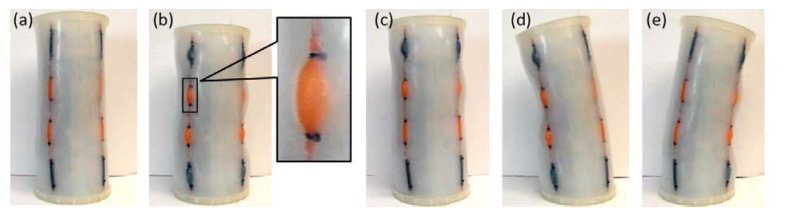
\includegraphics[width=\textwidth]{SoftSleeve.png}
    \caption[Soft sleeve prototype. (a) Original shape. (b) All muscles activated, contracting the whole body and amplified image of one muscle. (c) Partial contraction, only the 1st and 2nd top rows are activated. Both (d) and (e) illustrate bending movements, only two adjacent columns are activated.]{Soft sleeve prototype. (a) Original shape. (b) All muscles activated, contracting the whole body and amplified image of one muscle. (c) Partial contraction, only the 1st and 2nd top rows are activated. Both (d) and (e) illustrate bending movements, only two adjacent columns are activated \cite{Park2012}. }
    \label{fig:soft_sleeve}
\end{figure}

In recent works, the virtual anchor technique, a very novel concept which uses pneumatic artificial muscles is described \cite{wehner2013lightweight}. This concept, attempts to address the challenges on force transmission using soft materials attached or strapped to the skin, such as discomfort and slippage. The key anchor points of the human body are defined as the ones exhibiting large bony landmarks. These regions are capable of withstanding high forces and of minimizing the slippage or chaffing of soft materials positioning on them. The virtual anchor technique is also motivated by the changes in length of some parts of the skin surface during joint motion, where some parts exhibit more changes than others. The soft exosuit was developed by interconnecting PAMs and nylon straps, replicating the extensible and non-extensible paths of the skin, respectively, in the specific points where the changes in the skin length take place. These places are called virtual anchor points which in combination with the key anchor points allow a good transmission of forces without causing discomfort to the user. The concept is illustrated in \Cref{fig:anchor_concept}, where the orange lines represent the pneumatic actuators interconnected with the key anchors and the virtual anchors. These interconnections constrain the actuator movements other than the desired, as well as redirect the actuator reaction forces to the areas of the body capable of withstanding these forces. Finally, this design was able to reduce the metabolic cost caused by wearing the complete device (10 kg), by almost 100\%. Considering that no control system, other than a timed activation sequence, and no perception system was implemented, this technique opens the door for further improvements to achieve a better degree of assistance.

\begin{figure}[hbtp!]
    \centering
    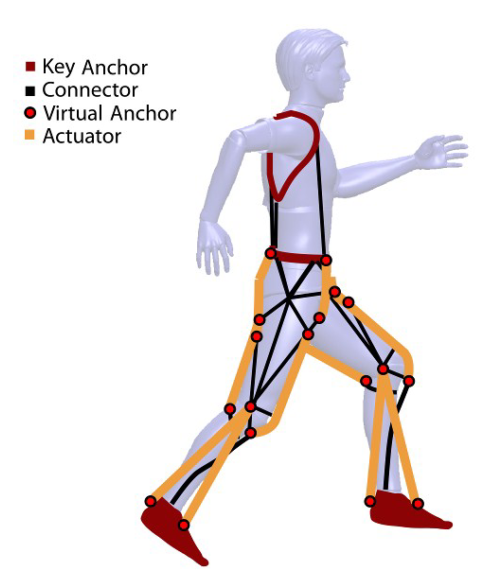
\includegraphics[width=0.45\textwidth]{AnchorConcept.png}
    \caption[Virtual anchor concept. The three key anchors (red square) located at the foot, hip and shoulder are interconnected with the soft actuators (orange) and auxiliary connectors (black) in specific points called virtual anchors (red circle) to stabilize the forces created by the actuators.]{Virtual anchor concept. The three key anchors (red square) located at the foot, hip and shoulder are interconnected with the soft actuators (orange) and auxiliary connectors (black) in specific points called virtual anchors (red circle) to stabilize the forces created by the actuators \cite{wehner2013lightweight}. }
    \label{fig:anchor_concept}
\end{figure}

Putting aside the McKibben-type actuators as the most common choice for pneumatic muscles, elastomers such as high-flexible silicone can be used to build PAMs as shown in \cite{Park2014}. This PAM consists of interconnected flat chambers made of silicone rubber which inflate when pressurized air is injected (\Cref{fig:Flat_elastomer}), the innovative concept in this work is the zero-volume air chamber which provides a higher degree of compliance and compactness (traditional PAMs retain air inside them even when they are not actuated). Kevlar fibres are embedded inside this soft actuator to constrain the expansion direction, creating a contraction movement when pressurized. The flatness of these actuators simplifies the casting process. Furthermore, the chamber-based design makes it possible to join each chamber together not only in series, which increases the contraction length, but in parallel as well to increase the contraction force. In order to test the actuator performance, a soft exosuit similar to the previously described was developed using nylon straps and hooks to connect the soft actuator to the points of interest. The developed soft orthosis, intended for infant-toddler rehabilitation, was capable of delivering a 38 N contraction force and 18 mm contraction length by implementing a muscle with an array of four elastomer actuators inter-connected in series. In addition, a total excursion for the knee joint of 132\textdegree{} was achieved, considering both flexion and extension motions (\Cref{fig:Flat_elastomer}). Moreover, in a most recent development by \cite{Low2016}, it can be found the implementation of elastomers for ankle assistance, in this case the pulling force of the PAM is generated when the actuator deflates and a pushing force is generated when it inflates, an inverted behaviour in comparison to previously mentioned applications. This soft orthosis consists of a regular sock which is attached to both ends of the PAM, that is enclosed into textile to restrict its longitudinal and radial expansion mainly. Despite the simplicity and assistance capabilities of the device, it cannot be worn with shoes, restricting the assistance to indoor activities
\begin{figure}[hbtp!]
    \centering
    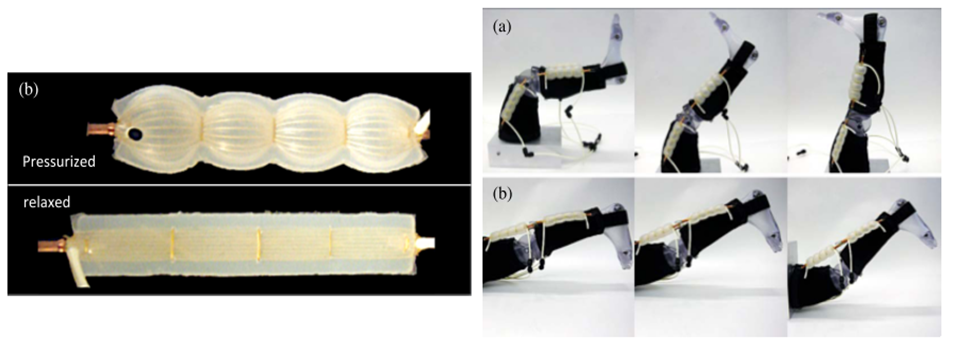
\includegraphics[width=1\textwidth]{FlatElastomer.png}
    \caption[(a) Flat elastomer pneumatic actuator in (1) pressurized and (2) relaxed states. (b) Implementation of the flat actuator in medical leg model assistance, along with the achieved (1) extension, and (2) flexion motion.]{(a) Flat elastomer pneumatic actuator in (1) pressurized and (2) relaxed states. (b) Implementation of the flat actuator in medical leg model assistance, along with the achieved (1) extension, and (2) flexion motion \cite{Park2014}. }
    \label{fig:Flat_elastomer}
\end{figure}

This concept, of expanding instead of contracting the PAM when pressurizing, is called Inverse PAM (IPAM). This soft actuator is called `Hydro Muscle', and is directly compared with McKibben muscles since it overcomes the main limitations of the latter. The main difference between this actuator and the previously mentioned is the shift from pneumatic technology to hydraulics, in fact, it is reported that the pressure found in homes tap water is enough to actuate it \cite{Sridar2016}. Therefore, the cylindrical shape `Hydro Muscle' is capable of elongating axially, increasing its stiffness radially, when pressurized; and of the exact opposite behaviour when depressurized (\Cref{fig:IPAM}). The actuator functionality is due to two structural layers of different materials. The inner layer is a tube made of an elastic material (latex showed better performance than the commonly used silicon) and the outer layer is made of a soft but inelastic material, such as polyester, which restricts the inner layer radial expansion and allows its axial expansion. Despite the simplicity of the design, this new concept of actuator is free of energy losses in radial expansion. Also, the energy losses inherent when using compressed air as the power source are not present in this design (in comparison to PAMs).
\begin{figure}[hbtp!]
    \centering
    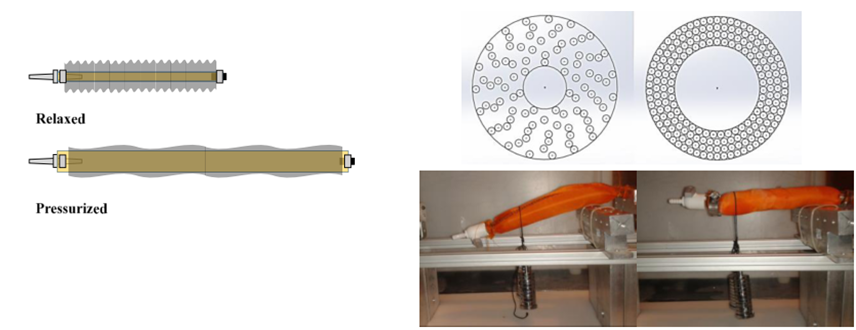
\includegraphics[width=\textwidth]{IPAM.png}
    \caption[(a) IPAM developed in its relaxed and pressurized state, the small radial expansion and large axial expansion is appreciated. (b) Cross-sectional view of the jamming effect ongoing inside the actuator, and (c) bending effect caused by heavy load, and correction of the bending using the jamming effect.]{(a) IPAM developed in its relaxed and pressurized state, the small radial expansion and large axial expansion is appreciated. (b) Cross-sectional view of the jamming effect ongoing inside the actuator, and (c) bending effect caused by heavy load, and correction of the bending using the jamming effect \cite{Sridar2016}. }
    \label{fig:IPAM}
\end{figure}

The experiments performed in this work showed that this innovative soft actuator is 33\% more efficient in comparison to a McKibben muscle using hydraulics. Furthermore, this actuator can be easily manufactured with off-the-shelf components. Nonetheless, the convenience of using both pneumatic and hydraulic muscles for performing pulling instead of pushing tasks, is to prevent the bending effect caused when the actuator is fixed in one of its ends and has a heavy load attached to the other end. The latter effect is amplified for pushing tasks being one of the main drawbacks of the proposed actuator concept. The solution to this is to use the principle of jamming by filling the gap between the inner and outer layer with granular media which will jam when the actuator is pressurized (\Cref{fig:IPAM}). Another IPAM which implements a very similar concept as the one illustrated in (\Cref{fig:IPAM}) can be found in \cite{Hawkes2016}. This IPAM managed to achieve a strain of 300\% of its length, which is three times more the achieved strain of the IPAM illustrated in (\Cref{fig:IPAM}). This improvement is achieved due to the complete restriction on the stretchable material in the inner layer to only expand along its axis and not radially. The main benefits of recent IPAMs in comparison with traditional PAMs are: high strain and nearly linear control (since no radial deformation is present). Finally, the ability to achieve high strains make IPAMs suitable for joints like the elbow.

\subsubsection{Cable-driven Actuators} \label{sec:cable-driven}

Another actuation technology implemented in soft orthoses is cable-driven actuators, based on electric motors, in combination with Bowden cables. Following the same principle as pneumatic muscles, this technology relies on generating tensions along a cable which, with a right positioning along the human lower limb, can transmit torques to the human body. The work in \cite{asbeck2013biologically} presents the design and implementation of a battery operated soft exosuit built with Bowden cables (\Cref{fig:bowden_exo}). 
\begin{figure}[hbtp!]
    \centering
    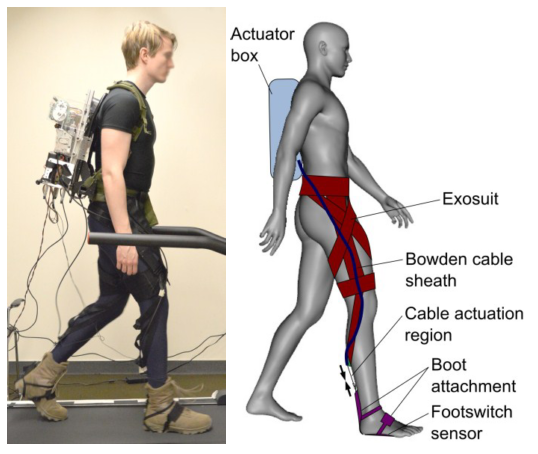
\includegraphics[width=0.5\textwidth]{BowdenExosuit.png}
    \caption[(a) Developed Bowden cable-based soft exosuit prototype. (b) Initial design concept highlighting the main parts of the soft exosuit.]{(a) Developed Bowden cable-based soft exosuit prototype. (b) Initial design concept highlighting the main parts of the soft exosuit \cite{asbeck2013biologically}. }
    \label{fig:bowden_exo}
\end{figure}

The exosuit is based on the leg's muscles functionality during normal walking, with the objective of assisting the forward propulsion stage of the gait. The soft exosuit structure made of fabrics is attached to the waist and above the knee, from the former the Bowden cable follows a path of webbing straps into the lower limb, ending at the ankle. In order to minimize the chaffing and displacement on the webbing strap structure caused by the tension on the cables while actuated, the strap along the waist of the user terminates at the hip which is a natural bony part of the human body. In other words, there is almost no muscle and fat tissue between the skin and the bone, which improves the transmission of forces without causing discomfort to the user. This soft exosuit delivers 18\% and 30\% of the torques required for normal walking on the knee and hip, respectively. However, despite the innovative design, the main limitation of this exosuit structure is the large displacement experienced on its structure, of 13 cm, when the cables are under tension. This displacement caused the cable-driven actuators to have a very low efficiency since almost 45\% of the generated mechanical power is lost in the form of friction forces in the soft exosuit structure. Nonetheless, the proposed multi-joint concept allows the actuation of two joints using a single actuator.

Following the multi-joint actuation concept, another soft exosuit is designed in \cite{Bartenbach2015} with the objective of not only providing assistance but also to enable impaired users. This concept, illustrated in (\Cref{fig:bowden_exo2}), exploits the benefits of using a single cable-driven actuator to control more than one joint, i.e. multi-joint actuation. The difference in this case is the deep analysis performed regarding the compatibility of the joints, taking into account synergy of torque and equal polarity of torque. In order to assist the desired movements of sit-to-stand, walking and stairs ascend, the knee and the hip joints were selected as the most suitable combination. Despite the limited scope of this work, being focused only on the concept design, the authors expect the selected joint combination to support the movements of sit-to-stand and stairs ascend.

\begin{figure}[hbt!]
    \centering
    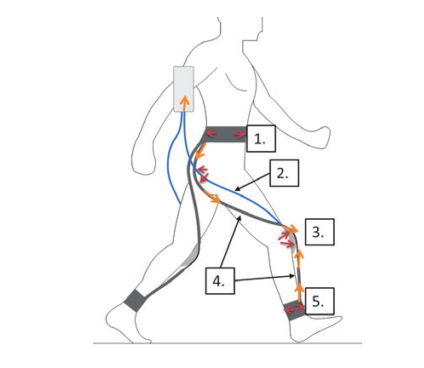
\includegraphics[width=0.7\textwidth]{BowdenExosuit2.png}
    \caption[Multi-joint actuated soft exosuit. There are two anchor points, one at the pelvis (1) and one at the shank (5). The suit is actuated by a bowden cable (2) and positioned at the front of the knee. The contractile element is connected connected to the two anchors by webbing elements (4). Knee module to increase the lever arm (3). Red arrows: reaction forces, and orange arrows: actuation force.]{Multi-joint actuated soft exosuit. There are two anchor points, one at the pelvis (1) and one at the shank (5). The suit is actuated by a bowden cable (2) and positioned at the front of the knee. The contractile element is connected connected to the two anchors by webbing elements (4). Knee module to increase the lever arm (3). Red arrows: reaction forces, and orange arrows: actuation force \cite{Bartenbach2015}. }
    \label{fig:bowden_exo2}
\end{figure}

The next follow up on the concept of multi-joint actuation is documented in \cite{Ding2014} where a testing platform for soft exosuits was developed. The aim of this platform is to study the performance of the multi-joint actuation concept when being implemented in different soft exosuits. The off-board platform integrates several cable-driven actuators and the sensors required to evaluate their performance. In addition, this platform can deploy sensors to be attached to the exosuit and compare relevant metrics such as mechanical power efficiency. This platform, which can be reconfigured to meet different applications, has been used to evaluate the advantages of implementing single joint and multi-joint actuation, highlighting the benefits of the latter \cite{Ding2016}. Furthermore, the study performed with the aid of this platform provided designing parameters for the development of an exosuit, in other words, the multi-joint platform assists the designing phase, ultimately reducing designing times.

\subsubsection{Shape Memory Materials}

The two main groups of shape memory materials implemented in soft robotics are: shape memory alloys (SMAs) and shape memory polymers (SMPs). Both technologies function under the same principle: they can switch to a different shape when a stimulus such as heat is in contact with them. Nevertheless, there are some differences to be mentioned. The SMAs have two main phases, one for high temperature (austenite) and one for low temperature (martensite), when they suffer deformation while being in the martensite phase they can recover from the deformation by exposing them to heat, therefore SMAs convert the energy from heat into mechanical energy to return to their original shape \cite{ImagesScientificInstrument2016}. This property is usually exploited to cause contraction changes in the material (\Cref{fig:SMA}). Therefore, SMAs are commonly used in combination with cable-driven actuators.
\begin{figure}[hbtp!]
    \centering
    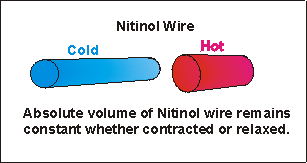
\includegraphics[width=0.5\textwidth]{SMA.png}
    \caption[Shape memory alloys made of Nitinol. The contraction effect under the increase in temperature is illustrated.]{Shape memory alloys made of Nitinol. The contraction effect under the increase in temperature is illustrated \cite{ImagesScientificInstrument2016}. }
    \label{fig:SMA}
\end{figure}

The implementation of SMAs into robotic applications have three main challenges to be addressed: response speed, high power consumption and low operational bandwidth. The functionality of SMAs is based on the property found in metals in which heat is generated when an electric current flows through it, this is also known as the Joule effect. Depending on the metals used in the alloy, the amount of heat required for the SMA to recover from deformation is high enough to melt plastics, this excess of energy is what makes SMAs inefficient \cite{Bundhoo2009a,Bundhoo2009}. Furthermore, SMAs have a very low response time due to the large amount of time required to cool them down, limiting their operation frequency. This limitation is only present when air convection is used as the cooling process. Due to this, SMAs have been found to be unsuitable for most orthoses in which an operating frequency of roughly 6 Hz is required. However, plenty of authors have successfully developed the latter devices, in both rigid \cite{tarkesh2007} and soft variations \cite{Stirling2011}, capable of assisting human motions. This proves the feasibility of using SMAs for applications such as clinical rehabilitation where slow and repetitive cycles are required \cite{Pittaccio2009,Chenal2014}. An example of these applications are: re-positioning, muscle toning, functional exercise and assistive robotics \cite{pittaccio2012shape,Coral2012}. Currently, extensive research is being done to address the main limitation of SMAs, as documented in \cite{Coral2012}.

J. Zhang proposed a novel SMA-based artificial muscle \cite{Zhang2013a}. This configuration facilitates the addition of a cooling system, due to the cylindrical hollow shape of the artificial muscle. Therefore, a mini pump is used to create a flow of air inside the artificial muscle, effectively reducing the cooling time by 10 times. The performance of this artificial muscle is further improved by considering the hysteresis behaviour typically found in SMAs when shifting between the low and high temperature phases. Furthermore, there is again evidence of trying to replicate the muscle-tendon functionality, in this case by adding a spring in series with the artificial muscle which aids the SMA recovery phase. The latter simulate a more realistic behaviour, similar to the human muscles behaviour. Moreover, this is the first documented work that deals with the modelling of the actuator behaviour, allowing the implementation of a robust control system which can be also used in other scenarios involving SMAs. Finally, this artificial muscle is deployed as part of an active foot orthosis capable of large contractile forces by using in parallel more than one SMA wire to form each of the pulling tendons (\Cref{fig:SMA_orthosis}). Low efficiency and low operational bandwidth were identified as the main drawbacks of this design.

\begin{figure}[hbtp!]
    \centering
    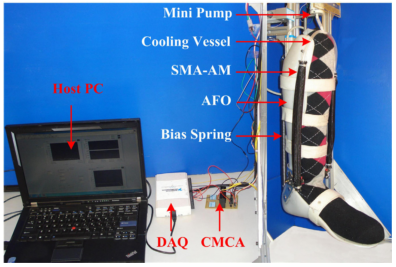
\includegraphics[width=0.7\textwidth]{SMAOrthosis.png}
    \caption[Ankle joint soft orthosis. The developed SMA artificial muscle along the main parts are highlighted.]{Ankle joint soft orthosis. The developed SMA artificial muscle along the main parts are highlighted. \cite{Zhang2013a}. }
    \label{fig:SMA_orthosis}
\end{figure}

Current SMAs are also limited by the amount of contraction they can achieve, i.e. operational bandwidth, which is commonly 3\% of its original length. Recent solutions to this, are based on deploying the SMAs in several loops, exploiting the same concept of using pulleys with cables, essentially increasing the usable length of the SMA wire without increasing the size of the final actuator. However, relying on pulleys in a soft actuator greatly reduces compliance, increases the actuator weight, and may cause twisting between the individual turns of the SMA wire. Therefore, a new approach described in \cite{Villoslada2015}, make use of the outer sheath of Bowden cables to contain the SMA wires inside. This concept allows the SMA to be directed in many ways to the point of interest, allowing the actuator to have different shapes that can be compliant with the user's body, e.g. the SMA can be wrapped around the user's arm in a solenoid-like shape which also increases the SMAs wire length (\Cref{fig:flexible_actuator}). Furthermore, pulleys are also implemented to allow the SMAs to have a maximum number of three turns contained inside the Bowden sheath. Two main drawbacks were discovered during an experimental testing: SMAs wires were twisting between each other which caused high friction losses and prevented the SMA to completely recover its initial length; the other drawback was the Bowden sheath material which was found to have low force transmission efficiency. In order to solve the latter, the Bowden cable sheath made of nylon was replaced by flexible tubes of Polytetrafluoroethylene (PTFE) and every SMA wire turn was individually encased in a narrow-gauge sheath. The final experiments showed that the developed actuator is capable to contract 9\% of its length which is three times the theoretical contraction length of an SMA wire.

\begin{figure}[hbtp!]
    \centering
    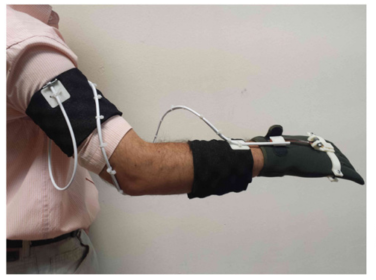
\includegraphics[width=0.5\textwidth]{FlexibleActuator.png}
    \caption[Flexible wrist exoskeleton prototype.]{Flexible wrist exoskeleton prototype. \cite{Villoslada2015}. }
    \label{fig:flexible_actuator}
\end{figure}

Shape memory polymers (SMPs) are a little bit more complex than SMAs. They have two main phases: a glassy state (high stiffness) and a rubbery state (low stiffness). Furthermore, when they are in their rubbery state, they can be deformed by applying small forces and preserve the deformation by cooling the SMP. In this state, the SMP can be considered rigid and it has to be heated to the point of the transition temperature to return to its original shape, hence having shape memory. This property of preserving a deformation is analysed by K. Takashima et al. in an attempt to boost the McKibben artificial muscle performance \cite{Takashima2010}. McKibben actuators are unable to maintain their contraction shape unless precise and continuous control is implemented which cause premature wear on controlling elements as well as higher energy consumption. Therefore, a SMP is embedded into the McKibben braid which, by controlling the SMP temperature, allows the artificial muscle to hold its contracted position as illustrated in \Cref{fig:mckibben}. It is worth mentioning that SMPs can be stimulating in different ways to obtain the change of shape, such as infrared light, electric field, magnetic field and even manipulating the material water content. In the previous work, the SMP was stimulated by heat and cooled down using a compressor, which drastically limits the actuator portability.

The benefits of SMPs, in comparison to SMAs, can be summarized as: lightweight, low cost, rigidity in low temperature and flexibility in high temperature, higher strains (around 400\% in comparison with 7\% for SMAs), and they can be easily moulded into 3D shapes. Furthermore, the main positive aspects of the improved McKibben artificial muscles are: allows rigidity fixing, the parameter to control stiffness can be used to control actuation, and controllability of the actuator surface by individually stimulating certain segments of the SMP.

\begin{figure}[hbtp!]
    \centering
    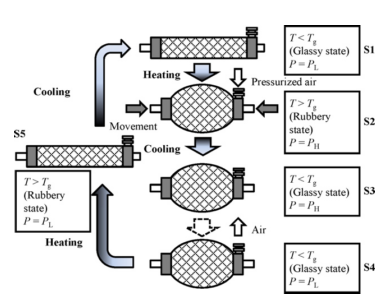
\includegraphics[width=0.8\textwidth]{Mckibben.png}
    \caption[Schematic illustrating McKibben with embedded SMP functionality. $T_g$: transition temperature, $P_H$: high pressure, $P_L$: low pressure.]{Schematic illustrating McKibben with embedded SMP functionality. $T_g$: transition temperature, $P_H$: high pressure, $P_L$: low pressure \cite{Takashima2010}. }
    \label{fig:mckibben}
\end{figure}

\subsection{Soft Perception Technologies}

Currently, the most common soft perception technologies are based on liquid metal alloys embedded into soft materials such as elastomers. These strain soft sensors are widely used in soft orthoses, such as the one in \cite{park2011bio}. The materials used in this case were Eutectic Gallium Indium (eGaIn), as the liquid metal alloy, and silicon rubber as the flexible layer, which creates a highly deformable sensor (\Cref{fig:strain_sensor}). The sensor was implemented to measure changes in the ankle joint proportional to the skin strain which it was attached to, by measuring the changes in resistance caused by the variations in the path length and cross-sectional area of the channel containing the liquid metal. Nevertheless, the developed soft orthoses implemented two other non-soft sensors: an inertial measurement unit (IMU) as an angle position detection and a pressure sensor attached to the shoe insole to detect foot strikes, hence the gait cycle. The developed strain sensor delivered good performance and contributed in the development of a feedback controller for this soft orthosis.

\begin{figure}[hbtp!]
    \centering
    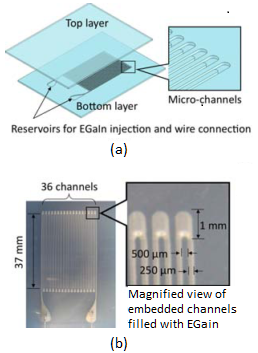
\includegraphics[width=0.6\textwidth]{StrainSensor.png}
    \caption[Soft strain sensor. The microchannel filled with liquid metal can be appreciated in: (a) concept design and (b) the prototype.]{Soft strain sensor. The microchannel filled with liquid metal can be appreciated in: (a) concept design and (b) the prototype \cite{park2011bio}. }
    \label{fig:strain_sensor}
\end{figure}

Liquid metal alloys are also implemented in \cite{Park2012}, as previously described, in the form of embedded muscle-sensor units (\Cref{fig:soft_sleeve_sensor}). The soft strain sensor was capable of estimating the contraction length of a pneumatic muscle by measuring its radial expansion. In order to preserve softness, thin flexible copper wires were embedded into the cylindrical soft orthosis to obtain the sensor readings.

\begin{figure}[hbtp!]
    \centering
    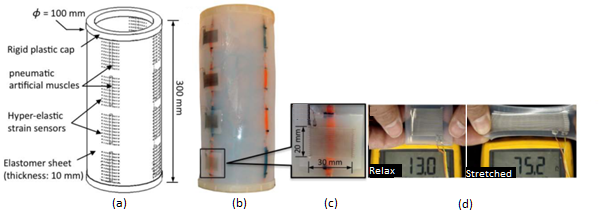
\includegraphics[width=0.9\textwidth]{SoftSleeveSensor.png}
    \caption[Soft sensor sleeve: (a) design concept, (b) developed prototype, (c) magnified view of the embedded sensor-actuator concept. (d) Soft strain sensor change in resistance during stretch and relax.]{Soft sensor sleeve: (a) design concept, (b) developed prototype, (c) magnified view of the embedded sensor-actuator concept. (d) Soft strain sensor change in resistance during stretch and relax \cite{Park2012}. }
    \label{fig:soft_sleeve_sensor}
\end{figure}

Taking the application of soft strain sensors with eGaIn a step further, a wearable soft suit capable of sensing the joint angles of the hip, knee and ankle joints, is presented in \cite{mengucc2013soft}. With the sensors properly positioned along the lower limb, by measuring the strain caused by the joint rotation, the joint angle can be known. The sensors tracked the user motions with a mean absolute error of 8\textdegree{}, being the most precise tracking achieved on the hip joint and the less precise on the ankle joint. In the mentioned work, only sagittal plane motions were measured, however, due to the great success and linearity of the sensors, they are planned to be implemented to measure motions in the frontal plane as well. The complete suit characterization can be found in \cite{mengucc2014wearable}, and is illustrated in \Cref{fig:Sensing_suit}.

\begin{figure}[hbtp!]
    \centering
    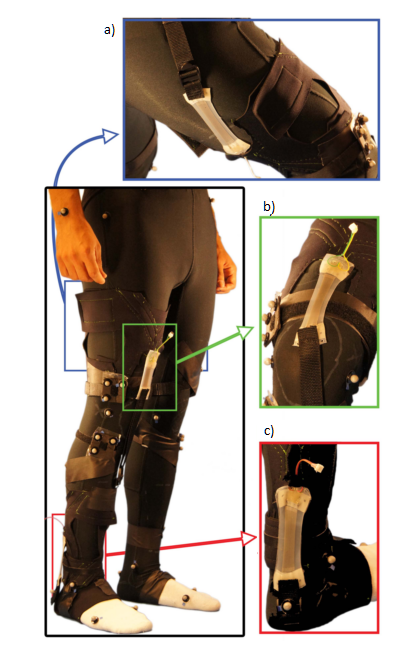
\includegraphics[width=0.4\textwidth]{SensingSuit.png}
    \caption[Implementation of soft strain sensors into a Soft sensing suit, (a) hip sensor, (b) knee sensor and (c) ankle sensor position.]{Implementation of soft strain sensors into a Soft sensing suit, (a) hip sensor, (b) knee sensor and (c) ankle sensor position \cite{mengucc2013soft}. }
    \label{fig:Sensing_suit}
\end{figure}

A potentially improved version of these soft strain sensors is presented in \cite{Chossat2013} where the highly stretchable elastomer is filled with two different conductive liquids, a traditional liquid metal and an ionic solution, instead of one. Interconnecting the strain soft sensor with the external application has been a big challenge, since the strain caused by the connection, usually soft wires, affects the sensor accuracy by increasing the total electrical resistance and by generating additional strain. Nevertheless, the ionic solution is intended to decouple the signal routing part from the sensing part to solve the latter challenge, creating a noise-free interface with the external application (\Cref{fig:hybrid_strain_sensor}).

\begin{figure}[hbtp!]
    \centering
    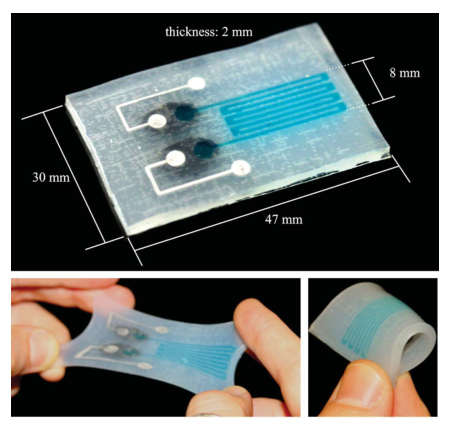
\includegraphics[width=0.5\textwidth]{HybridStrainSensor.png}
    \caption[Hybrid soft strain sensor, the interface between the liquid metal and the ionic solution can be clearly seen in dark areas.]{Hybrid soft strain sensor, the interface between the liquid metal and the ionic solution can be clearly seen in dark areas \cite{Chossat2013}. }
    \label{fig:hybrid_strain_sensor}
\end{figure}

One direct implementation of the embedded microchannel with conductive fluid sensors, can be seen in a recent improvement to the McKibben type PAM (\Cref{fig:braided_sensor}). McKibben actuators were widely adopted in soft robotics applications and there is plenty of information in the literature about their implementations. However, accurately sensing the deformation and force of these actuators still remains challenging. This has been addressed in many ways such as: cylindrical dielectric elastomers with carbon grease disposed on their surface to function as electrodes \cite{Goulbourne2007}; and also by attaching soft elastomer sheaths to the actuator, which are capable of sensing deformation due to their microchannels filled with conductive fluid \cite{Park2013}. The implementation of carbon grease electrodes and conductive microchannels allows the measuring of the actuator deformation. The conductive elements, mentioned before, change their electrical resistance when they are deformed. Furthermore, the concept of attaching these sensors to the actuator was refined in \cite{Felt2014,Felt2015}, where the sensing elements surrounding the actuator are now disposed in a helical shape. From the electric circuit created, it is possible to measure both the output force and length deformation of the actuator by correlating them with the circuit resistance and inductance respectively. This work proposed the implementation of conductive wires to build the reinforced braid of a McKibben actuator allowing the actuator to `sense', from there the given name of `Smart Braid', creating a solenoid-like circuit from which the inductance can be measured using a couple of mathematical approximations such as: the Neumann approximation and the long solenoid approximation, being the former one the most accurate and general; but at the same time the most expensive in terms of computation. The author exerts that this new sensing concept can be applied to multitude of scenarios in soft robotics, which includes soft orthosis.
\begin{figure}[hbtp!]
    \centering
    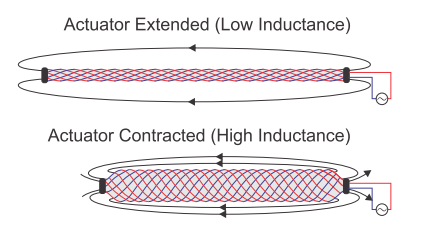
\includegraphics[width=0.5\textwidth]{BraidedSensor.png}
    \caption[`Smart Braid' concept. The variation in the actuator length cause a change in the electric circuit inductance.]{`Smart Braid' concept. The variation in the actuator length cause a change in the electric circuit inductance \cite{Felt2015}. }
    \label{fig:braided_sensor}
\end{figure}

\subsection{Control Technologies} \label{sec:controlSystems}

One of the successfully implemented control systems is documented in \cite{park2011bio}, which forms part of the previously mentioned concept illustrated in \Cref{fig:strain_sensor}. The control system is composed of several micro-controllers for parallel processing, and is divided in four main stages: sensing, signal processing, control and actuation (\Cref{fig:control_system}). The soft orthosis makes use of three different sensor technologies which requires different sampling and signal processing algorithms for each one, the IMU being the most complex one. Thereafter, another micro-controller with access to all the sensors, decides when to activate the solenoid valves that control the pneumatic muscles by generating pulse width modulated (PWM) signals. The latter describes a basic proportional control system. No mathematical model was deducted to describe the non-linear behaviour of the pneumatic muscles, instead, simpler controller approaches as feed-forward and feedback controller were implemented, with the latter being able to achieve a response time of 500 ms when a perturbation was present on the system, such as letting a weight hang from the device toe. The feedback controller made use of a soft strain sensor (\Cref{fig:strain_sensor}) to correct the ankle angle. Finally, although the controller performance is good it is still not enough to provide active gait assistance nor to predict user intentions. Another drawback is that the system requires calibration every time a new user wears it. Nevertheless, the developed soft orthosis is suitable for rehabilitation because it can achieve a dorsiflexion of 12\textdegree{} and 20\textdegree{} when foot was at resting position, and when foot was forced to a plantar flexion position, respectively. Moreover, the perception system could provide the clinician with meaningful data about the patient progress. The previous work was continued in \cite{park2014design} where a new controller was designed by considering the interaction between the soft exosuit and the human body as a black box, i.e. instead of trying to model the non-linear behaviour of the whole system some experiments were performed to obtain a system input/output relationship. Following this, classic control techniques were implemented to model a linear time-invariant controller. The results were promising since the original complex system performed adequately using simple techniques. Finally, the implementation of electromyography sensors was discussed to add the involuntary muscle contractions of the user into the system as a disturbance and improve the accuracy during different scenarios.

\begin{figure}[hbtp!]
    \centering
    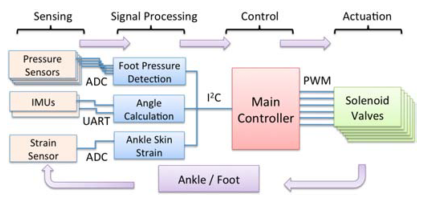
\includegraphics[width=0.7\textwidth]{ControlSystem.png}
    \caption[Control system architecture implemented for the ankle soft orthosis.]{Control system architecture implemented for the ankle soft orthosis \cite{park2011bio}. }
    \label{fig:control_system}
\end{figure}

In some cases, the design and development complexity of a control system for soft robotic applications limits the research to focus only on the implementation and study of the soft actuation and perception systems. This is the case for the work documented in \cite{Park2012}, the cylindrical soft sleeve with embedded muscle-sensor units. In the latter work, the developed controller is well designed but does not implemented a close-loop architecture nor complex mathematical models to predict the soft material behaviour.The control system consist of several micro-controller units, each of these communicated with their surrounding neighbours (\Cref{fig:soft_sleeve_sensor}). Each of the 16 nodes embedded into the cylindrical soft sleeve has a microcontroller unit with independent functionalities, such as recollecting and distributing the data. On top of this, there is a scheduling routine embedded in each unit which allows synchronization between them. Every unit has four tasks to execute at a given time and a given order: sensing, communicate, process data and actuate. The actuation parameters are generated using a mathematical approximation of the soft material behaviour which assumes no other deformation around the soft sleeve is caused by the compression of the pneumatic actuators. This assumption neglects the fact that when one side of the cylinder is under compression, the opposite side is under tension, i.e. the length on this side does not remain constant. The authors highlighted the necessity for a better approximation method when analysing the experimental results. For a desired bending angle of 15\textdegree{}, an actual bending angle of 11.5\textdegree{} was achieved. In simulation, feeding the soft sensors data into the mathematical approximation, a bending of 13\textdegree{} was estimated, which translates into an accuracy of 76\%.

The fact that few soft exosuit developments fully implement a control system does not imply that no research is being performed in the field. The implementation of current soft actuators into functional devices, as well as the proof of concept of emerging soft actuators are usually followed by an extensive study about modelling their behaviour to translate that information into a control system. On the field of PAMs, many interesting new approaches are being researched, such as implementing fuzzy logic techniques to improve their performance \cite{Chang2015,Skorina2015,Bishop-Moser2015,Hosovsky2016}. The next step in the research cycle of all soft actuation technologies is to implement the tested models into functional devices, which then will allow new concepts to be developed, hence new modelling research to be performed.

\section{Biomechanics of the Human Lower Limb}

The biomechanics of the human lower limb are self-contained between three planes of action, which are the sagittal plane, the frontal plane and the transverse (horizontal) plane \cite{PhysicalSolutions2016}. In combination with these planes there are three axes used to identify specific motions: frontal horizontal axis, vertical axis and sagittal horizontal axis. The positioning of each of them is illustrated in \Cref{fig:body_planes_axes}. The sagittal plane divides the body vertically into left and right parts, the frontal plane divides the body vertically into front (posterior) and back (anterior) parts and the transverse plane divides the body horizontally into upper (superior) and lower (inferior) parts. This coordinate system allows the many motions of each joint in the human body to be clearly identified.

\begin{figure}[htbp!]
	\centering
	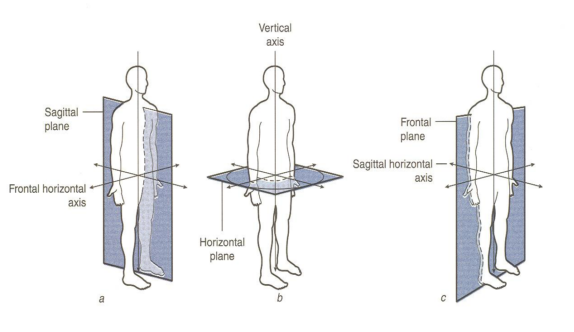
\includegraphics[width=\textwidth]{BoydPlanesAxes.png}
	\caption[Dimensional spaces used to understand human motions: (a) Sagittal plane, (b)Horizontal plane and (c)Frontal plane.]{Dimensional spaces used to understand human motions: (a) Sagittal plane, (b)Horizontal plane and (c)Frontal plane \cite{PhysicalSolutions2016}. }
	\label{fig:body_planes_axes}
\end{figure}

\newpage
The motions of each joint are named with respect to the plane and axis where they happen. This allows the easy recognition of the human body motions (\Cref{fig:lower_motion}). The biomechanics of the lower limb are categorized in five groups, each containing two individual motions, as follows:
\begin{itemize}
	\item Flexion and extension describe the bending motion which decreases, or increases the angle between two parts of the body, respectively.
	\item Abduction and adduction describe the motion away from, or towards the body midline, respectively.
	\item Eversion and inversion of the foot describe the motion away from, or towards the body midline, respectively.
	\item External rotation and internal rotation describe the motion away from, or towards the body midline, respectively.
	\item Horizontal abduction and adduction describe the motion away from, or towards the body midline, respectively.
\end{itemize}

\begin{figure}[htbp!]
	\centering
	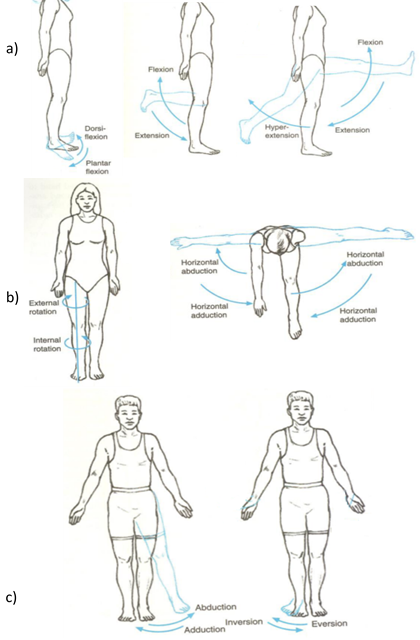
\includegraphics[width=0.8\textwidth]{LowerLimbMotionTerminology.png}
	\caption[Lower limb motions for (a) sagittal plane, (b) horizontal plane and (c) frontal plane.]{Lower limb motions for (a) sagittal plane, (b) horizontal plane and (c) frontal plane. Image adapted from  \cite{PhysicalSolutions2016}. }
	\label{fig:lower_motion}
\end{figure}

\newpage

\section{The Muscle-tendon Component} \label{sec:muscle_tendon}

Having defined the terminology involved in the biomechanics of the human skeletal muscle system, this section focuses on describing the muscle-tendon component from a mechanical point of view. In the literature, the mechanical model commonly used to describe the mechanical behaviour of the muscle-tendon component is the Hill's model \cite{hill1938heat}. This model is considered the most representative of all the available models \cite{zhang2012sma}. Hill's model describes the skeletal muscle as a three elements system, which contains a contractile element, a passive element, and a series element. The contractile element (CE) represents the muscle fibres in charge of generating the contractile forces, the parallel (passive) element (PE) is formed by the tissue surrounding the muscle which prevents it from over stretching, and the series element (SE) represents the human tendon, as illustrated in \Cref{fig:hillModel}.

\begin{figure}[htb!]
	\centering
	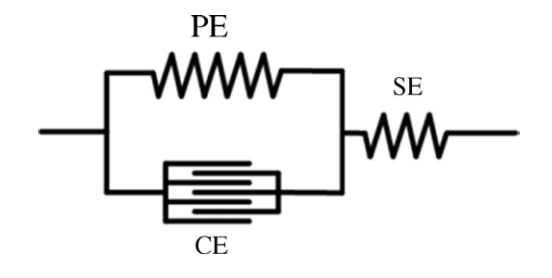
\includegraphics[width=0.4\textwidth]{HillModel.png}
	\caption[Hill's model of the skeletal muscle. The contractile element (CE), the parallel element (PE) and the series element (SE) are shown.]{Hill's model of the skeletal muscle. The contractile element (CE), the parallel element (PE) and the series element (SE) are shown \cite{hill1938heat}. }
	\label{fig:hillModel}
\end{figure}

Hill's model makes the important assumption of considering the SE to be purely elastic, i.e. the deformation of the element is entirely dependent on the force applied to it. Nevertheless, the non-linear viscoelastic properties of the human tendon are acknowledged in his work. The latter simplification is a common practice among studies of the skeletal muscle system because the muscle and tendon are studied as a whole (muscle-tendon component) \cite{zajac1989muscle}. Evidence of the actual benefits of this simplification is found in the literature for the field of robotics exoskeletons. The complex muscle-tendon model developed in \cite{lloyd2003emg}, considered the viscoelastic properties of the human tendon to estimate forces and joint torques in real time. The model achieved high accuracy at the cost of high computational load. In an attempt to reduce the computational load, the assumption of an infinitely stiff tendon was made which proved to be reliable as well \cite{sartori2009stiff}.

In a similar way, developments in the field of soft robotics which are inspired in the skeletal muscle system functionality are also based in Hill's model, as highlighted in \Cref{sec:SoftActuation}. Commonly, springs \cite{park2011bio} or Bowden cables \cite{Zhang2013a} are implemented as the SE of the muscle-tendon model. Nevertheless, the fact is that the human tendon has viscoelastic properties \cite{maurel1998biomechanical}. Most of the documented literature is mainly focused on developing and testing soft materials to be used as the contractile element in soft artificial muscles. The latter, previously identified as a research opportunity, indicates that the viscoelastic properties of soft materials have not been studied with the aim of developing a soft artificial tendon, which in combination with current soft artificial muscles could deliver better performance in soft robotic applications for human assistance.

Tendons are connective tissues that link muscles with bones. They have a non-linear viscoelastic behaviour, i.e. the proportional relationship between the reaction force experimented by the tendon and the applied deformation is not constant throughout the whole range of possible deformations. This reaction force is also dependent on the history of previous deformations. At rest, the collagen fibres (core components of tendons) are in a relaxed wavy state. When the tendon experiences a tensile force, the collagen fibres are easily stretched and realigned, opposing little resistance to deformation. However, when the collagen fibres are completely stretched they begin to offer more resistance to deformation which is proportional to the applied force. Finally, fibres can be stretched to their limit and failure of the tendon will occur \cite{nordin2001basic}. This non-linear response to the applied deformation is better explained using \Cref{fig:tendonSS} where the characteristic S-shape curve for a tendon stress-strain curve is appreciated.

\begin{figure}[htb!]
	\centering
	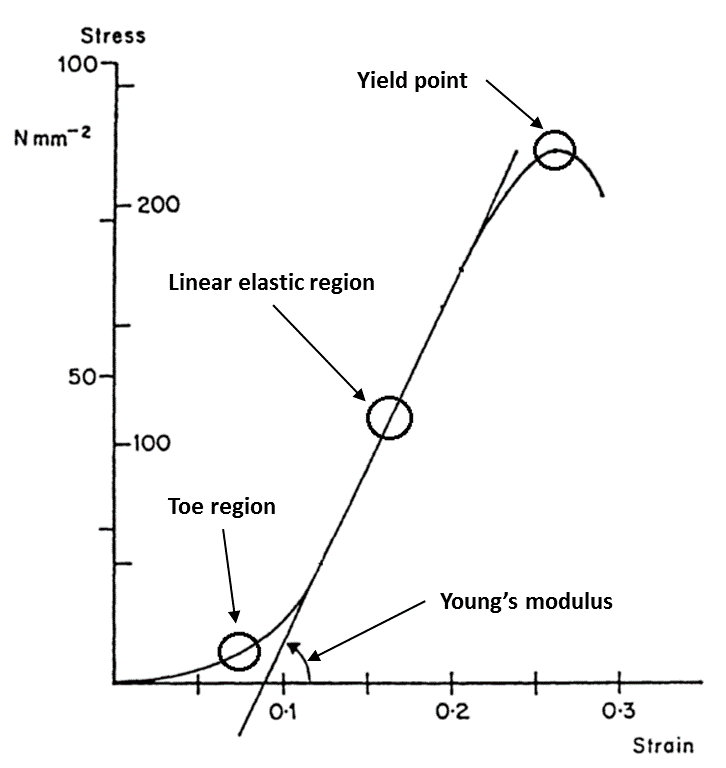
\includegraphics[width=0.6\textwidth]{TendonStressStrain.png}
	\caption[Tendon stress-strain curve.]{Tendon stress-strain curve. Image adapted from \cite{maurel1998biomechanical}. }
	\label{fig:tendonSS}
\end{figure}

The stress-strain curve in \Cref{fig:tendonSS} illustrates the mechanical properties of a human tendon. The stress is described as the tensile force per cross-sectional unit area experienced by the tendon. This stress causes the tendon to elongate. In the chart, the elongation is represented as the strain, which is the tendon deformation in relation to its original length. Along with the stress-strain curve, the force-elongation curve is also used to visualize the mechanical properties of tendons. These experiments are performed in a static state, i.e. the strain rate is the same throughout the whole experiment. Therefore, they do not provide any information about the viscoelastic properties of the tendon.

Viscoelastic materials exhibit both elastic and viscous characteristics. Viscosity describes a fluid's resistance to flow, the more viscous a fluid is, the more slowly it will flow and vice versa. The latter suggests a time-dependent behaviour. In the case of viscoelastic materials, this time-dependent behaviour is shown when subjecting the material to different rates of strain or deformation. For example, the stress-strain curve of the human tendon, illustrated in \Cref{fig:tendonSS}, would have a greater slope in the elastic region if a greater strain rate is applied. The viscoelastic behaviour of the human tendon can be analysed with the following mechanical tests: stress relaxation, creep (deformation over time) and hysteresis \cite{nordin2001basic}.

During the stress relaxation experiment, the tendon is subjected to a constant deformation (length remains the same throughout the whole experiment). To avoid plastic deformations, i.e. incorrect measurements, the parameter of deformation for this experiment must not exceed the linear region of the material. The initial force/stress triggered as a response of the applied deformation will decrease over time (relax) until reaching equilibrium. From this experiment a chart of force against time is generated (\Cref{fig:tendonSR_Creep}). In a similar way, in the creep experiment a constant force is applied to the material. The material will creep as time passes, in other words, the deformation caused by the applied force will increase over time until reaching equilibrium. A chart of deformation against time is generated (\Cref{fig:tendonSR_Creep}). Finally, during the hysteresis experiment the tendon is subjected to cyclic tests where a load is applied up to a certain stress level and then released (unloading). The tendon behaviour shows two different paths, one for loading and one for unloading. Due to the time-dependent behaviour of viscoelastic materials, each cycle will generate different load-unload paths since the time interval for each cycle to be executed are intentionally defined to prevent the material from reaching equilibrium (\Cref{fig:tendonHysteresis}).

\begin{figure}[htb!]
	\centering
	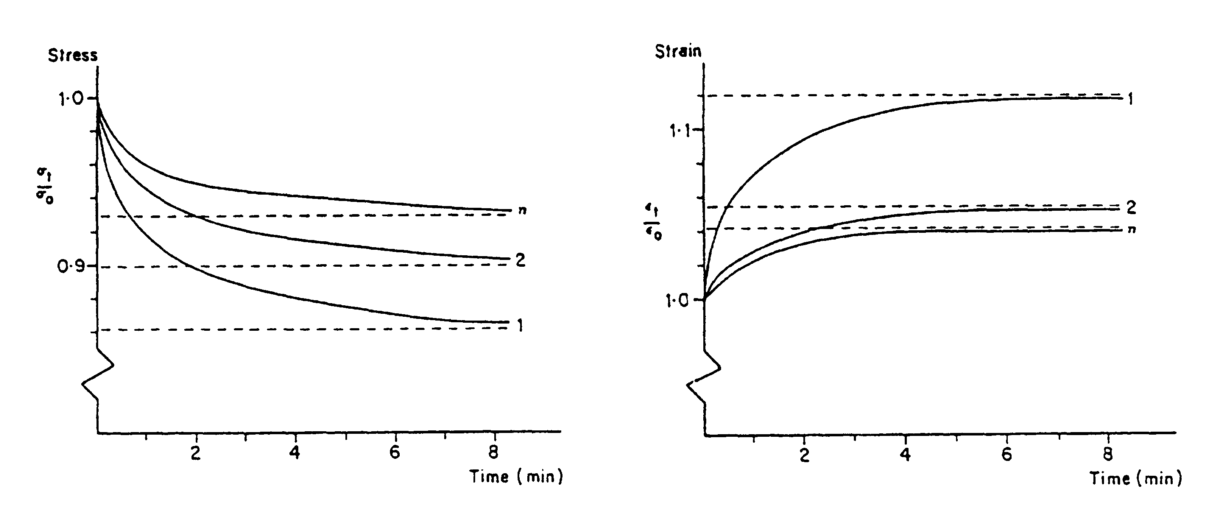
\includegraphics[width=\textwidth]{TendonSR&Creep.png}
	\caption[Tendon curves for the experiments of: (a) stress relaxation and (b) creep. The experiments were executed several times under the same conditions, the curve labelled \textit{n} illustrates the tendon reaching a steady state where repeatability between experiments is achieved.]{Tendon curves for the experiments of: (a) stress relaxation and (b) creep. The experiments were executed several times under the same conditions, the curve labelled \textit{n} illustrates the tendon reaching a steady state where repeatability between experiments is achieved. Image reproduced from \cite{maurel1998biomechanical} }
	\label{fig:tendonSR_Creep}
\end{figure}

\begin{figure}[htb!]
	\centering
	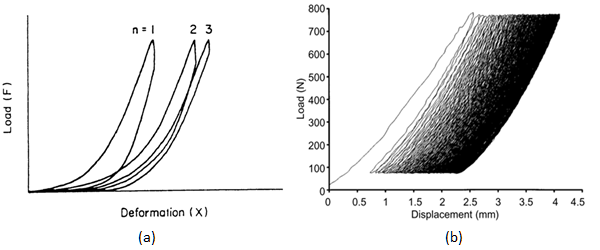
\includegraphics[width=\textwidth]{TendonHysteresis.png}
	\caption[Hysteresis of the human tendon. (a) Deformation chart shows both loading and unloading paths for few cycles and (b) displacement chart shows 200 loading-unloading cycles. The preconditioned state of the tendon is reached for cycles above 50.]{Hysteresis of the human tendon. (a) Deformation chart shows both loading and unloading paths for few cycles and (b) displacement chart shows 200 loading-unloading cycles. The preconditioned state of the tendon is reached for cycles above 50. Images taken from \cite{maurel1998biomechanical,schatzmann1998effect} respectively. }
	\label{fig:tendonHysteresis}
\end{figure}

When performing mechanical experiments to find the tendon properties at failure, the obtained results are different between a preconditioned and an unconditioned tendon, as proved in \cite{schatzmann1998effect}. This effect is illustrated in \Cref{fig:tendonSR_Creep} as well, for both experiments, the tendon relaxation and creep are smaller for each new testing cycle until reaching an equilibrium state, i.e. the preconditioning state. The previous set of experiments is useful to characterize the non-linear viscoelastic properties of tendons and soft materials. 

\section{Modelling Tools for Soft Materials } \label{sec:modelingTechniques}

The majority of the soft robotic applications implement soft materials from the family of thermoplastic elastomers (TPE). These type of materials are known to have a non-linear stress response, low stiffness, high deformation lengths, time-dependent and temperature-dependent stress response \cite{Bauman2008}. These mechanical properties are similar to the ones found in biological skin or muscle tissue. Due to this, soft materials are being implemented in soft robotic applications. However, it is imperative to have a reliable modelling technique to fully take advantage of the viscoelastic properties of soft materials.

The stress response of soft materials, such as TPE is non-linear and viscoelastic. The majority of the documented modelling approaches to predict the viscoelastic behaviour of soft material is based on the development of a mathematical constitutive model. The Linear Viscoelastic Models (LVMs) are commonly used for this task \cite{xu2014mathematical,tirella2014strain,lu2017constitutive,ciniello2017identifying}. This is also the case when for the modelling of biological tissues \cite{sanjeevi1982viscoelastic}. The LVMs are a set of mathematical models that use two basic components, a spring and a dashpot, in different configurations and quantities to describe the viscoelastic mechanical behaviour of materials \cite{roylance2001engineering}. Inside this family of mathematical models, there are a couple of them which, in theory, can describe the viscoelastic behaviour of any material, as long as the required number of parameters is met. This immediately imposes the restriction of having enough computational power to deal with the model complexity when high accuracy is required.

The implementation of soft materials in soft robotic applications for human assistance has recently gained more attention. Most of the efforts are focused on improving the traditional series-elastic actuator (SEA) by replacing its elastic element, commonly a metallic spring, with a viscoelastic material, such as rubber. SEAs are from the family of cable-driven actuators and are commonly paired with electric motors. The main feature of these actuators is that they have an elastic element between the actuator and the load. SEAs have greatly impacted the field of robotics, specifically in legged robotics and powered orthoses, due to many benefits such as: greater shock tolerance, low output impedance, passive energy storage, and better force feedback accuracy \cite{pratt1995series,pratt2004series,au2008powered}. SEAs are now a mature actuation technology, and as such, they have a well-defined trade-off, caused by the fixed stiffness provided by linear springs traditionally used. More often than not, variable stiffness is more suitable for legged robots and powered orthoses. The latter limitation have been addressed by developing variable stiffness actuators \cite{groothuis2012vsaut}, using non-linear metallic springs \cite{migliore2007novel}, and very recently by using viscoelastic materials, such as polymers and rubber \cite{rollinson2013design,parietti2011series,schepelmann2014compact}. However, most of these works, still face the challenge of accurately modelling the mechanical behaviour of soft materials. 

In \cite{parietti2011series}, where the concept of a series-viscoelastic actuator (SVA) is first mentioned, the modelling of the soft material is based on the Burger Model, one of the most complete LVMs, in combination with a controlling technique known as the state space observer. The accuracy of the system was found to be proportional to the complexity of the mathematical model used. The studied material in this work was a rigid-acrylic based photopolymer (FullCure720). The reported control system contained the viscoelastic model, the state space observer, and a cascaded force-velocity scheme, in other words, a very complex and well thought control system for a linear viscoelastic polymer. The developed SVA is illustrated in \Cref{fig:firstSVA}. 

\begin{figure}[htb!]
	\centering
	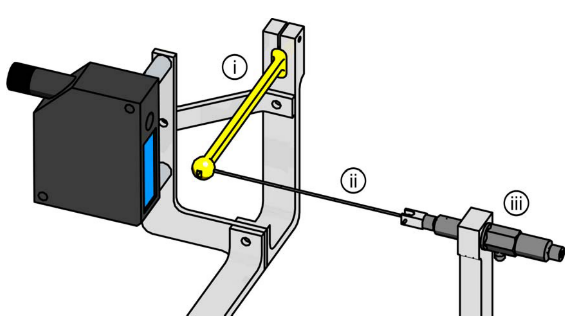
\includegraphics[width=0.6\textwidth]{FirstSVA.png}
	\caption[Series-viscoelastic actuator proposed by Parietti et al. The end-effector is rigidly mounted on the revolving lever (i), which also supports the laser sensor. A Nylon line (ii) connects the end-effector handle to the high-precision piezoelectric force sensor (iii), which is fixed to a rigid support.]{Series-viscoelastic actuator proposed by Parietti et al. The end-effector is rigidly mounted on the revolving lever (i), which also supports the laser sensor. A Nylon line (ii) connects the end-effector handle to the high-precision piezoelectric force sensor (iii), which is fixed to a rigid support \cite{parietti2011series}.}
	\label{fig:firstSVA}
\end{figure}

Following this line of research, Rollinson et al. attempted to add viscoelasticity to a SEA, this time a soft material is used, natural rubber, instead of a rigid polymer \cite{rollinson2013design}. The developed SEA has a rotary spring. Two different types of rubber, and a type of neoprene, were studied. In here, the stress response of the materials is considered linear and instead, the hysteresis of the material is modelled. Again, the modelling of the soft material is based on one of the LVMs, the Standard Linear Solid (SLS) model, which is slightly less complex than the Burger model. Thanks to the proposed mechanical design for the rotary SEA, the reported stress response of the studied rubbers was surprisingly linear under a specific range of deformations. The authors concluded that more work is required to create better modelling techniques for the hysteresis and non-linear behaviour of soft materials like elastomers. The developed rotary spring is illustrated in \Cref{fig:rotarySoftSEA}.

\begin{figure}[htb!]
	\centering
	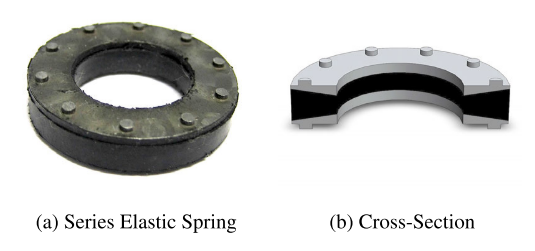
\includegraphics[width=0.6\textwidth]{RotarySoftSEA.png}
	\caption[Developed soft rotary spring: (a)photo and (b)cross-section.]{Developed soft rotary spring: a)photo and b)cross-section \cite{rollinson2013design}.}
	\label{fig:rotarySoftSEA}
\end{figure}

Following a more traditional approach, Schepelmann et al. incorporated viscoelasticity in cable-driven SEA by using a rubber material as the elastic element, instead of the traditional metallic spring \cite{schepelmann2014compact}. In here, no LVMs are used, instead the non-linear stress response of the rubber is simplified by fitting a second order exponential curve to the stress-strain curve of the material. The main motivation of this work is to tackle the limitations of SEA with non-linear springs (NLS), where computer-aided manufactured (CAM) structures are used to define a known deflection trajectory of the spring, thus defining a torque trajectory. Essentially, CAM structures can relate the spring deformation with the generated torque, allowing the implementation of control systems. This work successfully validated the suitability of rubber to be incorporated as part of a SEA (\Cref{fig:softSEACAM}). However, under the limited range of testing parameters, the authors were not able to observe any velocity-dependency on the stress response of the rubber. In the conclusions, a state space observer is recommended to improve the accuracy of the reported forces transmitted by the soft material, i.e. to allow the controller to compensate the hysteresis and non-linear stress response of the material.

\begin{figure}[htb!]
	\centering
	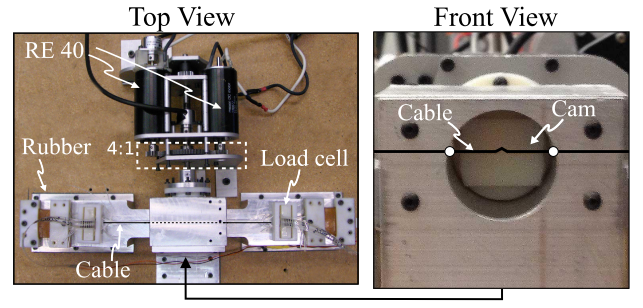
\includegraphics[width=0.6\textwidth]{SoftSEACAM.png}
	\caption[Benchtop setup for rubber characterization and observer testing. The load side of the rubber is fixed. Load cells in-line with the rubber give rubber force measurements for testing. The choice of electric motors and transmission is illustrated.]{Benchtop setup for rubber characterization and observer testing. The load side of the rubber is fixed. Load cells in-line with the rubber give rubber force measurements for testing. The choice of electric motors and transmission is illustrated \cite{schepelmann2014compact}.}
	\label{fig:softSEACAM}
\end{figure}

In an attempt to relieve the controller for such load, the latter work was continued by Austin et al. in \cite{austin2015control}, this time the focus was on developing a modelling tool to better describe the complex behaviour of rubber. In here, the complexity of modelling the non-linear and strain-dependent stress response of soft materials is addressed, for the first time, by upgrading the SLS model without greatly increasing its complexity. A 
piecewise linearisation is implemented, to transform the equilibrium spring in the SLS model into several springs in parallel which sequentially engages in proportion to the strain applied to the material. The developed mathematical model is called the Standard Linear Solid model with Strain-Dependent Stiffness. (Std. Lin. SDS). Although, the SLS is not the most complete model among the LVMs, the reported accuracy of the developed model is impressive. The control system implemented a state space observer, as well, which was capable of estimating the torque generated by the rubber spring. However, despite the large improvement in accuracy obtained by the developed Std. Lin. SDS, the hysteretic properties of the rubber lead to instability at higher frequencies, suggesting that there is still work to be done in this field.

\section{Summary} \label{sec:gaps}

The available literature suggests a growing interest in the research and development of soft actuation technologies, soft perception systems, and control systems to pair with the latter two. Also, and following the bio-inspiration driving the field of Soft Robotics, many works are attempting to imitate the capabilities of the human musculoskeletal system by developing soft actuators capable of behaving like the human muscle-tendon component. This is more evident when looking at the available works on Pneumatic Artificial Muscles (PAMs) where the actuator is used as the contractile force generator element (muscle), and a flexible interface (tendon) is used to transmit that force to the desired location. Similarly, established technologies such as electric motors, which can deliver forces in both directions of rotation, are being used in combination with Bowden cables to create pulling forces. This type of setup is known as a redundant system because more than one actuator is required to control both directions of rotation of a joint. Moreover, the research and development of new soft materials, such as the SMA and SMP, are also focused on creating materials that can contract when stimulated. There is still plenty of work to be done in this matter, which is why this is identified as one gap in the body of knowledge.

The majority of the literature is focused on testing a new soft actuation concept in an open-loop environment, i.e. with no control system implemented. This is caused by the fact that modelling the mechanical behaviour of a soft material is very complex. Even the control system of the most documented work in the literature, the ankle-foot orthosis, does not implement a modelling technique to monitor the behaviour of the PAMs, instead it is focused on extracting as many information as possible from the environment and to use this to decide when and how to activate the PAM \cite{park2011bio}. The literature dealing with the control systems of soft robotic applications is limited. Recently, attempts of adding viscoelasticity to well-established actuation technologies have been done. Specifically, viscoelasticity has the potential to address many of the limitations found in series-elastic actuators. The available literature on the subject is scarce but very well documented. In general, the reviewed works face a common challenge, the modelling of the viscoelastic properties of the materials used to accurately estimate their reaction force or torque. Rubber is the most common choice in these applications. Almost all of the documented modelling approaches are based on the Linear Viscoelastic Models, for the prediction of the material behaviour. However, the work performed by Austin et al. in \cite{austin2015control}, is the first attempt to upgrade the potential of the LVMs using a Piecewise linearisation method. The authors succeeded in developing a mathematical model, called the Standard Linear Solid model with Strain-Dependent Stiffness. (Std. Lin. SDS) which achieved higher accuracy than traditional models. However, even with the aid of controlling techniques such as the state space observer, the implemented control system is still incapable of accounting for properties of the material, such as hysteresis and the velocity-dependency in their stress response. Nevertheless, the developed mathematical model has the potential to be upgraded further by using the same Piecewise linearisation method but on a more complex LVM. The latter clearly indicates a growing interest in this field of research, its importance and a current gap in the body of knowledge.

Therefore, two main gaps are considered in the body of knowledge which are addressed by this research. On the one hand, more research is required to understand the functionality of the human musculoskeletal system, and to develop a soft actuation technology which mimics the functionality of the muscle-tendon component. On the other hand, there is a lack of reliable modelling tools to predict the complex mechanical behaviour of soft materials being used in soft actuation technologies.

%According to the literature, the most commonly implemented soft actuation technologies in soft robotic applications for human assistance are: Pneumatic/hydraulic artificial muscles, cable-driven actuators based on electric motors, and shape memory alloys/polymers.  In cable-driven actuators, the amount of generated assistance is proportional to the electric motor mechanical output power. This means, large forces can be generated to even enhance the user capabilities, yet again, the transmission of these forces via the human body prevents this enhancement. A common problem is the relative displacement of the soft structure worn by the user when tensile forces are generated by the pulling action of Bowden cables. Nevertheless, one advantage of this technology in soft exosuits is the `remote' actuation capability, which means that the electrical motors can be placed distal to the joint to be assisted, concentrating the weight of the heavy parts of the soft exosuit in convenient locations of the human body, e.g. as a backpack. Another advantage of this technology is the flexibility of the Bowden cables which allows them to be deployed in many different trajectories along the human body, facilitating the use of the body parts capable of sustaining high forces.

%In contrast, the other two soft technologies are commonly placed proximal to the joint to be assisted, which might allow a better distribution of the soft orthosis weight. Recent works have tackled the main limitations of PAMs, SMA and SMP. Particularly, big improvements have been achieved for PAMs and SMA. For the case of PAMs, the traditional and extensively implemented McKibben type muscle have been improved in terms of performance by the development of the Inverse PAM (IPAM). This latter technology surpasses the McKibben type muscle in assistance capabilities, efficiency and controllability. Furthermore, the concept of the IPAM can also be implemented using hydraulics which again comes with several advantages, a crucial one, the amount of generated force. The main disadvantage of both pneumatic and hydraulic actuators is the need for a compressor unit, which greatly decreases the soft orthosis autonomy and portability. Nevertheless, the recently developed `Hydro Muscle', which uses pressurized water from a home tap, greatly increases the appealing of this technology. In a similar way, the greater efficiency of IPAMs allows portable tanks with pressurized air to be used.

%The situation is quite similar for SMAs, many of the limitations from this technology, such as low strain, slow speed response and complex controllability have been addressed and improved. However, this technology is still in its early stages and their main drawbacks are high energy consumption and large amounts of generated heat, which makes them unsafe for human assistance applications. In the field of soft sensors, one of the main advantages of the soft strain sensors is that they can be custom-built to fit any application. When characterizing these sensors, two parameters are always mentioned: the electrical resistance and the gauge factor, the latter relates the strain with the change in resistance. Despite their original purpose of measuring strain changes, they can be used for angle measurements. On the controller side, the amount of research being performed in modelling the complex behaviour of soft actuators is slowly but constantly increasing. Nevertheless, the complexity of tackling the latter is evidenced in the scarce literature available.

%In summary, this literature review highlighted a very specific and bio-inspired trend in soft robotic applications for human assistance, which is mimicking the human musculoskeletal system, specifically the muscle-tendon component. This approach is very compatible with soft technologies that are commonly placed proximal to the assisted joint (PAMs, SMAs, IPAMs, etc.), and many soft artificial muscles have already been developed. These works, however, have mainly focused on the contractile element of the muscle-tendon component, leaving plenty of room to research about the viscoelastic element, the tendon. The most straightforward way to study the potential benefits of mimicking the human tendon behaviour is to incorporate soft materials to current soft actuation technologies as part of the mechanism to transmit generated forces. Essentially, creating a soft artificial tendon. Nevertheless, the success of maturing the previous concept into a soft robotic application greatly depends on having a reliable modelling tool which predicts the mechanical behaviour of soft materials. Finally, as mentioned in \Cref{sec:gaps}, this research aims to address two main gaps in the body of knowledge. On the one hand, the lack of literature about the implementation of soft materials as part of the force transmitting mechanism, which could allow for a better mimicking of the human musculoskeletal system. On the other hand, the lack of a modelling tools capable of predicting the mechanical behaviour of soft materials.
